\documentclass{article}

\usepackage{graphicx} % for images
\usepackage{amsmath} % for math
\usepackage{amssymb} % for \mathbb
\usepackage{siunitx} % for \SI, \num
\usepackage{hyperref} % for \url{}

% This stuff is for figures
\usepackage{float}
\DeclareGraphicsExtensions{.pdf, .png, .jpg}

% coloring of links for PDF format
\hypersetup{
    colorlinks=true,
    urlcolor=blue,
    linkcolor=blue
}

% \c command redefinition (for monospaced font)
\renewcommand{\c}[1]{\texttt{#1}}
% \today command re-definition
% https://tex.stackexchange.com/questions/112932/today-month-as-text
\renewcommand{\today}{\ifnum\number\day<10 0\fi \number\day \space%
\ifcase \month \or January\or February\or March\or April\or May%
\or June\or July\or August\or September\or October\or November\or December\fi\space%
\number \year} 

\begin{document}

\noindent
Rodrigo Becerril Ferreyra\\
Dr. Alireza Mehrnia\\
Homework 3\\
\today

The code used to generate the following results can be found at the end of this document.

%\addcontentsline{toc}{section}{P2.2}

\section*{P3.1}
Below are the plots of magnitude and argument for the DTFT of the given sequences.
\begin{figure}[H]
    \centering
    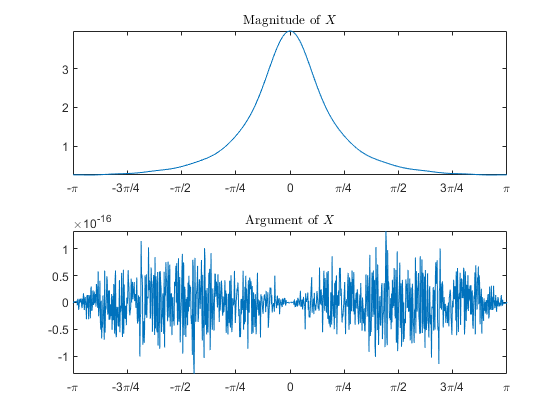
\includegraphics[width=\textwidth]{html/Homework3_01.png}
    \caption{Problem 3.1 Part 1}
    \label{3.1.1}
\end{figure}
Note how this DTFT has very little (negligible) argument; for all purposes, the DTFT is purely real.

\begin{figure}[H]
    \centering
    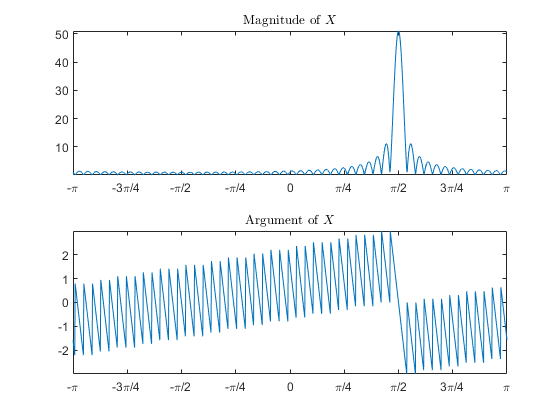
\includegraphics[width=\textwidth]{html/Homework3_02.png}
    \caption{Problem 3.1 Part 3}
    \label{3.1.3}
\end{figure}
Note how both the magnitude and argument seem to be centered around \(\pi/2\).

\section*{P3.3}
The following DTFTs were found analytically (using the definition of DTFT), then plotted using MATLAB. The definition is as follows:
\begin{equation}
    \mathcal{F}(x[n]) = X\left(e^{j\omega}\right) = \sum_{n = -\infty}^\infty x[n] e^{-j\omega n}
\end{equation}
\subsection*{Part 2}
In this example, \(x[n] = 0.6^{|n|}( u(n+10) - u(n - 11) )\), which has the following graph. Note that the value is zero at all indexes \(n < -10\) and \(n > 10\), where \(n\) is the index.
\begin{figure}[H]
    \centering
    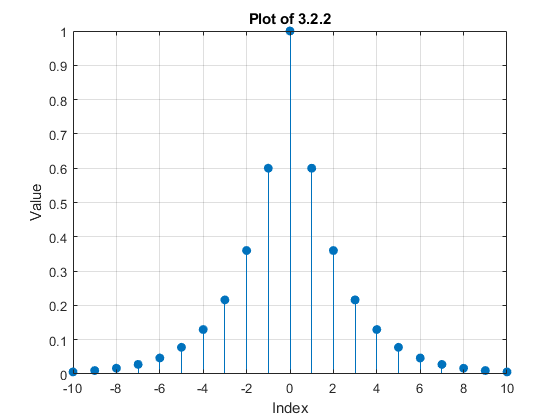
\includegraphics[width=\textwidth]{Images/Problem-3-2-2.png}
    \caption{Graph of \(x[n]\).}
    \label{plot 3.2.2}
\end{figure}

Below is the calculation for the DTFT.
\begin{gather*}
    \mathcal{F}[0.6^{|n|}( u(n+10) - u(n - 11) )] \\
    = X\left(e^{j\omega}\right) = 
    \sum_{n = -10}^{10} 0.6^{|n|}e^{-j\omega n}\\
    = 0.6^{10}e^{10j\omega} + 0.6^{9}e^{9j\omega} + 0.6^{8}e^{8j\omega} + 0.6^{7}e^{7j\omega} + 0.6^{6}e^{6j\omega}\\ + 0.6^{5}e^{5j\omega} + 0.6^{4}e^{4j\omega} + 0.6^{3}e^{3j\omega} + 0.6^{2}e^{2j\omega} + 0.6e^{j\omega} + 1\\
    + 0.6e^{-j\omega} + 0.6^2e^{-2j\omega} + 0.6^3e^{-3j\omega} + 0.6^4e^{-4j\omega} + 0.6^5e^{-5j\omega}\\ + 0.6^6e^{-6j\omega} + 0.6^7e^{-7j\omega} + 0.6^8e^{-8j\omega} + 0.6^9e^{-9j\omega} + 0.6^{10}e^{-10j\omega}
\end{gather*}

\begin{figure}[H]
    \centering
    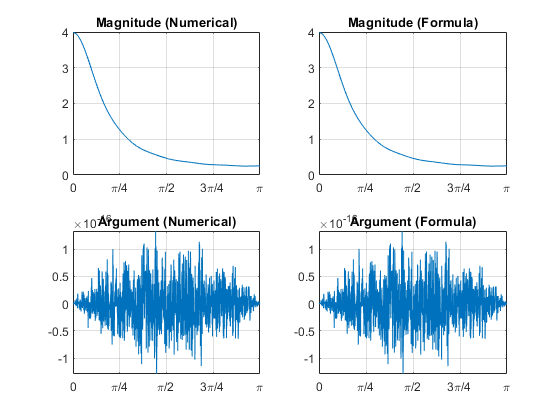
\includegraphics[width=\textwidth]{html/Homework3_03.png}
    \caption{Problem 3.3 Part 2}
    \label{3.3.2}
\end{figure}

\subsection*{Part 5}
In this example, \(x[n] = 4(-0.7)^n \cos(0.25\pi n)u(n)\). The
graph of this is below.
\begin{figure}[H]
    \centering
    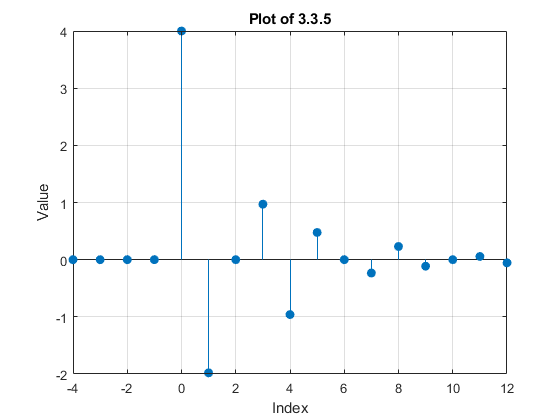
\includegraphics[width=\textwidth]{Images/Problem-3-2-5.png}
    \caption{Graph of \(x[n]\).}
    \label{plot 3.3.5}
\end{figure}

Below is the calculation for the DTFT.
\begin{align*}
    X\left(e^{j\omega}\right) &= \sum_{n=0}^\infty 4(-0.7)^n\cos(0.25\pi n)e^{-j\omega n}\\
    &=\sum_{n=0}^\infty 2(-0.7)^n \left(e^{j0.25\pi n} + e^{-j0.25\pi n}\right)e^{-j\omega n}\\
    &=\sum_{n=0}^\infty 2(-0.7)^n
    \left(
        e^{j\pi n/4} e^{- j\omega n} + e^{-j\pi n/4} e^{- j\omega n}
    \right)\\
    &=\sum_{n=0}^\infty \left( 2
        (-0.7)^n e^{j\pi n/4} e^{- j\omega n} +2 (-0.7)^n e^{-j\pi n/4} e^{- j\omega n}
    \right)\\
    &= \sum_{n=0}^\infty 2
    (-0.7)^n e^{j\pi n/4} e^{- j\omega n} +
    \sum_{n=0}^\infty 2 (-0.7)^n e^{-j\pi n/4} e^{- j\omega n}\\
    &= \sum_{n=0}^\infty 2
    \left[(-0.7) e^{j\pi/4} e^{- j\omega}\right]^n +
    \sum_{n=0}^\infty 2 \left[(-0.7) e^{-j\pi/4} e^{- j\omega}\right]^n\\
    &= \frac{2}{1 + 0.7 e^{j\pi/4} e^{- j\omega}}
    + \frac{2}{1 + 0.7 e^{-j\pi/4} e^{- j\omega}}
\end{align*}

The summation reduction formula \(\sum_{n=0}^\infty ar^n = \frac{a}{1-r}\) only works if \(|r| < 1\); in this case, since \(r\) is the complex number \((-0.7)e^{\pm j\pi/4 - j\omega}\), its magnitude \(|r| = 0.7\), making the summation reduction valid.

\begin{figure}[H]
    \centering
    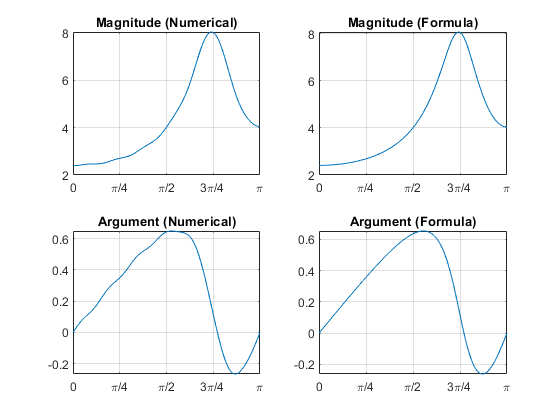
\includegraphics[width=\textwidth]{html/Homework3_04.png}
    \caption{Problem 3.3 Part 5}
    \label{3.3.5}
\end{figure}

\section*{P3.4}
Below is the plot for the rectangular window function for \(M = 50\). Other values of \(M\) can be obtained via the code.
\begin{figure}[H]
    \centering
    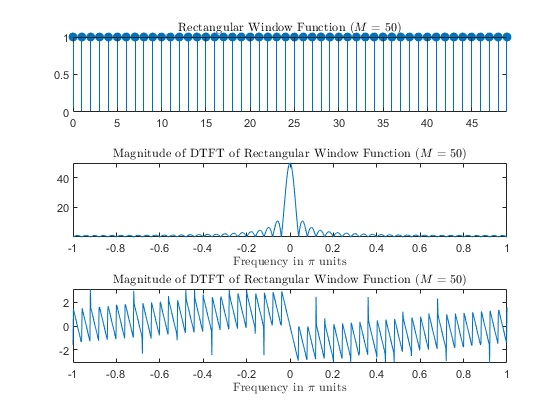
\includegraphics[width=\textwidth]{html/Homework3_07.png}
    \caption{Problem 3.4 Part 1}
    \label{3.4.1}
\end{figure}

Similarly, below is the plot for the rectangular window function for \(M = 50\). Other values of \(M\) can be obtained via the code.
\begin{figure}[H]
    \centering
    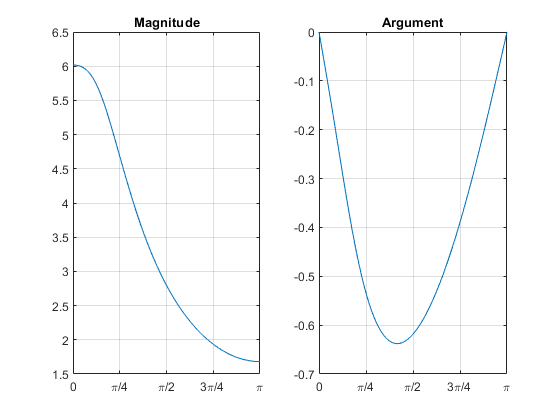
\includegraphics[width=\textwidth]{html/Homework3_17.png}
    \caption{Problem 3.4 Part 4}
    \label{3.4.4}
\end{figure}

\section*{P3.5}
Since the DTFT is an invertible transformation, one can find the original signal \(x[n]\) given the transform \(\mathcal{F}(x[n])\).
\subsection*{Part 1}
\begin{gather*}
    X\left(e^{j\omega}\right) = 3 + 2\cos(\omega) + 4\cos(2\omega)\\
    = 3 + 2\left(\frac{e^{j\omega} + e^{-j\omega}}{2}\right) + 4\left(\frac{e^{2j\omega} + e^{-2j\omega}}{2}\right)\\
    = 3 + e^{j\omega} + e^{-j\omega} + 2e^{2j\omega} + 2e^{-2j\omega}\\
    = 2e^{2j\omega} + e^{j\omega} + 3 + e^{-j\omega} + 2e^{-2j\omega}\\
    x[n] = \{2, 1, \underset{\uparrow}{3}, 1, 2\}
\end{gather*}
\begin{figure}[H]
    \centering
    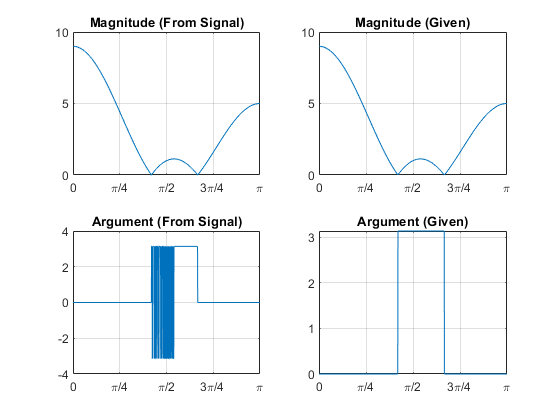
\includegraphics[width=\textwidth]{html/Homework3_13.png}
    \caption{Problem 3.5 Part 1}
    \label{3.5.1}
\end{figure}
\subsection*{Part 2}
\begin{gather*}
    X\left(e^{j\omega}\right) = \left[ 1 - 6\cos(3\omega) + 8\cos(5\omega) \right]e^{-3j\omega}\\
    = \left[1 - 6\left( \frac{e^{3j\omega} + e^{-3j\omega}}{2} \right) + 8\left(\frac{e^{5j\omega} + e^{-5j\omega}}{2}\right)\right] e^{-3j\omega}\\
    = \left[1 - 3e^{3j\omega} - 3e^{-3j\omega} + 4e^{5j\omega} + 4e^{-5j\omega}\right]e^{-3j\omega}\\
    = e^{-3j\omega} - 3e^{3j\omega - 3j\omega} - 3e^{-3j\omega - 3j\omega} + 4e^{5j\omega - 3j\omega} + 4e^{-5j\omega - 3j\omega}\\
    = e^{-3j\omega} - 1 - 3e^{-6j\omega} + 4e^{2j\omega} + 4e^{-8j\omega}\\
    = 4e^2j\omega - 1 + e^{-3j\omega} -3e^{-6j\omega} + 4e^{-8j\omega}\\
    x[n] = \{4, 0, \underset{\uparrow}{-1}, 0, 0, 1, 0, 0, -3, 0, 4\}
\end{gather*}
\begin{figure}[H]
    \centering
    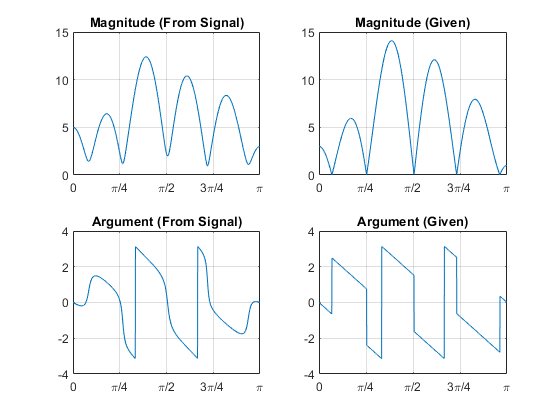
\includegraphics[width=\textwidth]{html/Homework3_14.png}
    \caption{Problem 3.5 Part 2}
    \label{3.5.2}
\end{figure}
\subsection*{Part 4}
\begin{gather*}
    X\left(e^{j\omega}\right) = \left[1 + 2\cos(\omega) + 3\cos(2\omega)\right]\cos(\omega/2)e^{-5j\omega/2}\\
    = \cos(\omega/2)e^{-5j\omega/2} + 2\cos(\omega)\cos(\omega/2)e^{-5j\omega/2} + 3\cos(2\omega)\cos(\omega/2)e^{-5j\omega/2}\\
    = \cos(\omega/2)e^{-5j\omega/2} + \left[ \cos(\omega/2) + \cos(3\omega/2) \right]e^{-5j\omega/2}\\ + \frac32\left[\cos(3\omega/2) + \cos(5\omega/2)\right]e^{-5j\omega/2}\\
    = 2\cos(\omega/2)e^{-5j\omega/2} + \cos(3\omega/2)e^{-5j\omega/2}\\ + \frac32 \cos(3\omega/2)e^{-5j\omega/2} + \frac32 \cos(5\omega/2)e^{-5j\omega/2}\\
    = \left(e^{j\omega/2} + e^{-j\omega/2}\right)e^{-5j\omega/2} + \frac12\left(e^{3j\omega/2} + e^{-3j\omega/2}\right)e^{-5j\omega/2}\\ + \frac34\left(e^{3j\omega/2} + e^{-3j\omega/2}\right)e^{-5j\omega/2} + \frac34\left(e^{5j\omega/2} + e^{-5j\omega/2}\right)e^{-5j\omega/2}\\
    = e^{-2j\omega} + e^{-3j\omega} + \frac12 e^{-j\omega} + \frac12 e^{-4j\omega} + \frac34 e^{-j\omega} + \frac34 e^{-4j\omega} + \frac34 + \frac34 e^{-5j\omega}\\
    = \frac34 + \frac54e^{-j\omega} + e^{-2j\omega} + e^{-3j\omega} + \frac54 e^{-4j\omega} + \frac34 e^{-5j\omega}\\
    x[n] = \left\{\underset{\uparrow}{\frac34}, \frac54, 1, 1, \frac54, \frac34\right\}
\end{gather*}
\begin{figure}[H]
    \centering
    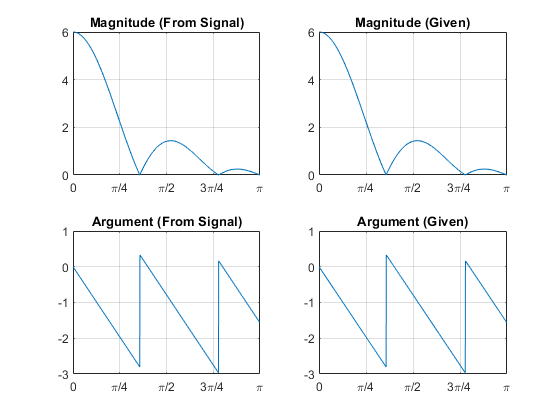
\includegraphics[width=\textwidth]{html/Homework3_15.png}
    \caption{Problem 3.5 Part 4}
    \label{3.5.4}
\end{figure}
\section*{P3.6}
The definition of the inverse DTFT is as follows:
\begin{equation}
    \mathcal{F}^{-1}[\mathcal{F}[x[n]]] = \mathcal{F}^{-1}\left[X\left[e^{j\omega}\right]\right] \equiv \frac1{2\pi} \int_{-\pi}^\pi X\left(e^{j\omega}\right)e^{j\omega n}\,d\omega
\end{equation}

\subsection*{Part 1}
\begin{gather*}
    X\left(e^{j\omega}\right) =
    \begin{cases}
        1 & \text{if } 0 \le |\omega| \le \pi/3\\
        0 & \pi/3 \le |\omega| \le \pi
    \end{cases}\\
    x[n] = \frac{1}{2\pi} \left[ \int_{-\pi}^{-\pi/3}0\,d\omega + \int_{-\pi/3}^{\pi/3}e^{j\omega n}\,d\omega + \int_{\pi/3}^\pi 0\,d\omega \right]\\
    = \frac{1}{2\pi} \int_{-\pi/3}^{\pi/3}e^{j\omega n}\,d\omega = \frac{1}{2\pi} \left[\frac{e^{j\omega n}}{0+jn}\right]_{\omega = -\pi/3}^{\omega = \pi/3} \\
    = \frac{1}{2\pi} \left( \frac{e^{jn\pi/3}}{ne^{j\pi/2}} - \frac{e^{-jn\pi/3}}{ne^{j\pi/2}} \right)\\
    = \frac{e^{j\left(n\pi/3 - \pi/2\right)} - e^{j\left(-n\pi/3 - \pi/2\right)}}{2\pi n}
\end{gather*}

\subsection*{Part 5}
\begin{gather*}
    X\left(e^{j\omega}\right) = \omega e^{j\left(\pi/2-10\omega\right)}\\
    x[n] = \frac{1}{2\pi} \int_{-\pi}^{\pi} \omega e^{j\left(\pi/2-10\omega\right)} e^{j\omega n}\,d\omega\\
    =\frac{1}{2\pi} \int_{-\pi/2}^{\pi/2} \omega e^{j\left(\pi/2-10\omega - \omega n\right)}\,d\omega\\
    =\frac{1}{2\pi} \left[\left. \frac{\omega e^{j\left(\pi/2 - 10\omega - \omega n\right)}}{-j\left(10 +n\right)}\right|_{-\pi}^{\pi}- \int_{-\pi}^\pi \frac{e^{j\left(\pi/2 - 10\omega - \omega n\right)}}{-j\left(10 +n\right)}\,d\omega \right]\\
    \frac{1}{2\pi} \left[ \frac{\pi e^{j\left(-19\pi/2 - \pi n\right)}}{-j\left(10 +n\right)} + \frac{\pi e^{j\left(21\pi/2 + \pi n\right)}}{-j\left(10 +n\right)}\right.\\
    \left. - \left. \frac{e^{j\left(\pi/2 - 10\omega - \omega n\right)}}{\left(-j\left(10 +n\right)\right)^2} \right|_{-\pi}^\pi\right]\\
    = \frac{e^{j\left(-19\pi/2 - \pi n\right)}}{-2j\left(10 +n\right)} + \frac{e^{j\left(21\pi/2 + \pi n\right)}}{-2j\left(10 +n\right)}\\
    +\frac{e^{j\left(-19\pi/2 - \pi n\right)}}{\left(100 + 20n + n^2\right)} - \frac{e^{j\left(21\pi/2 - \pi n\right)}}{\left(100 + 20n + n^2\right)}
\end{gather*}

\section*{P3.11}

\subsection*{Part 1}
\begin{gather*}
    h(n) = 0.9^{|n|}\\
    \mathcal{F}[h(n)] = H\left(e^{j\omega}\right) = \frac{1 - 0.9^2}{1 - 2(0.9)\cos(\omega) + 0.9^2}\\
    = \frac{0.19}{1.81 - 1.8\cos(\omega)}
\end{gather*}
This result was found using the given DTFT pairs.
\begin{figure}[H]
    \centering
    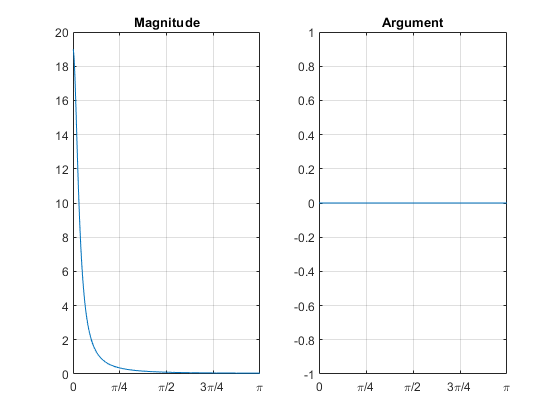
\includegraphics[width=\textwidth]{html/Homework3_16.png}
    \caption{Problem 11 Part 1}
    \label{3.11.1}
\end{figure}
\subsection*{Part 5}
\begin{gather*}
    h(n) = 0.5^{|n|}\cos(0.1\pi n)\\
    \mathcal{F}[h(n)] = \sum_{n=-\infty}^\infty 0.5^{|n|}\cos(0.1\pi n) e^{-j\omega n}\\
    =\frac12 \sum_{n=-\infty}^\infty 0.5^{|n|} \left(e^{0.1\pi n j} + e^{-0.1\pi n j}\right)e^{-j\omega n}\\
    =\frac12 \sum_{n=-\infty}^\infty 0.5^{|n|} \left[ \left(e^{0.1\pi j - j\omega}\right)^n + \left( e^{-0.1\pi j - j\omega} \right)^n \right]\\
    =\frac12 \sum_{n=0}^{-\infty} \left[\left(0.5e^{j\left(0.1\pi  - \omega\right)}\right)^n + \left(0.5e^{j\left(-0.1\pi  - \omega\right)}\right)^n \right]\\
    +\frac12 \sum_{n=0}^{ \infty} \left[\left(0.5e^{j\left(0.1\pi  - \omega\right)}\right)^n + \left(0.5e^{j\left(-0.1\pi  - \omega\right)}\right)^n \right]\\
    - 1 \text{ (this is because we're adding n=0 twice)}\\
    =\frac12 \sum_{n=0}^{\infty} \left[\left(0.5e^{j\left(0.1\pi  - \omega\right)}\right)^{-n} + \left(0.5e^{j\left(-0.1\pi  - \omega\right)}\right)^{-n} \right]\\
    +\frac12 \sum_{n=0}^{ \infty} \left[\left(0.5e^{j\left(0.1\pi  - \omega\right)}\right)^n + \left(0.5e^{j\left(-0.1\pi  - \omega\right)}\right)^n \right]
    - 1\\
    = \frac{1}{1-0.5e^{j\left(0.1\pi  - \omega\right)}} + \frac{1}{1-0.5e^{j\left(-0.1\pi  - \omega\right)}}\\
    + \frac{1}{1-0.5e^{j\left(0.1\pi  - \omega\right)}} + \frac{1}{1-0.5e^{j\left(-0.1\pi  - \omega\right)}} - 1\\
    = \frac{2}{1-0.5e^{j\left(0.1\pi  - \omega\right)}} + \frac{2}{1-0.5e^{j\left(-0.1\pi  - \omega\right)}} - 1
\end{gather*}
\begin{figure}[H]
    \centering
    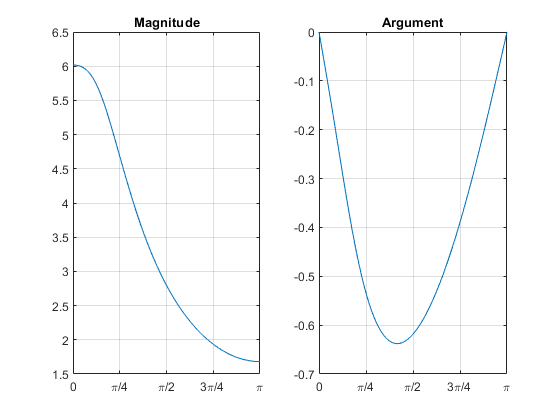
\includegraphics[width=\textwidth]{html/Homework3_17.png}
    \caption{Problem 11 Part 5}
    \label{3.11.5}
\end{figure}
\end{document}
